\documentclass{standalone}

\usepackage[OT1]{fontenc}
\renewcommand*\familydefault{\sfdefault}
\usepackage{helvet,sfmath}
\usepackage{siunitx}

\usepackage{tikz}
\usetikzlibrary{arrows,calc,patterns}
\usepackage{tikz,tkz-euclide}

\definecolor{BlueDefault}{rgb}{0.2,0.2,0.7}

\begin{document}

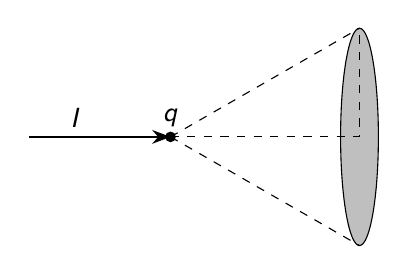
\begin{tikzpicture}[scale=0.6]
    %Current
    \draw[thick, -Stealth] (-3,0) to (0,0);
    \draw (-2,0) node[above]{\(I\)};
    %Charge
    \draw[fill = black] (0,0) circle (0.1);
    \draw (0,0) node[above]{\(q\)};
    %surface
    \draw[ fill = lightgray] (4,0) ellipse (0.4 and 2.3);
    \draw[dashed] (0,0) to (4,2.3);
    \draw[dashed] (0,0) to (4,-2.3);
    \draw[dashed] (0,0) to (4,0) to (4,2.3);
\end{tikzpicture}

\end{document}